\documentclass[12pt]{article}

%\documentclass[a4paper]{article}
\usepackage[utf8]{inputenc}
%\usepackage[paperwidth=210mm,left=20mm,right=20mm,top=20mm,bottom=20mm, paperheight=297mm, includefoot, heightrounded]{geometry}
\usepackage{pdfpages}
\usepackage{tikz}
\usepackage{enumitem}
\usepackage[acronym]{glossaries}

\usepackage{amssymb} %for fancy L
\usepackage{calrsfs} %for fancy L
\usepackage{cancel}
\usepackage{tabularx}
\usepackage[hyphens]{url}
\usepackage{booktabs}
\usepackage{graphicx}
\usepackage[titletoc,title]{appendix}
\usepackage{subfig}
\DeclareMathAlphabet{\pazocal}{OMS}{zplm}{m}{n} %for fancy L
\usepackage{epsfig, float,array,tabu,longtable,}
\usepackage{hyperref,wrapfig}
\usepackage{enumerate}
\usepackage{graphicx,psfrag}
\usepackage{cite}
\usepackage{sectsty}
\usepackage{epstopdf}
\usepackage{amsmath,esint, setspace, fancyhdr, amsfonts, bookmark, blindtext}
\usepackage[normalem]{ulem}
\usepackage{tikz}
\usepackage{rotating}
\usepackage[americanvoltages,fulldiodes,siunitx]{circuitikz}
\usepackage{stackengine}
\usetikzlibrary{matrix}
\usepackage{multirow}
\usepackage{multicol}
\usetikzlibrary{shapes,backgrounds,patterns}
\usetikzlibrary{mindmap,trees,decorations.markings}
\usetikzlibrary{quotes,angles}
\usepackage{lipsum}
\usepackage{verbatim}
\usepackage{geometry}
\renewcommand{\baselinestretch}{1}
\setlength{\textheight}{8.7in}
\setlength{\textwidth}{6.5in}

\setlength{\headheight}{0in}
\setlength{\headsep}{0.25in}
\usepackage{graphicx}
\setlength{\topmargin}{0in}
\setlength{\oddsidemargin}{0in}
\setlength{\evensidemargin}{0in}
\setlength{\parindent}{.3in}
\usepackage{listings}
\usepackage{color} %red, green, blue, yellow, cyan, magenta, black, white
\definecolor{mygreen}{RGB}{28,172,0} % color values Red, Green, Blue
\definecolor{mylilas}{RGB}{170,55,241}
\doublespacing

\include{acronyms_definitions}
\makeglossaries


\begin{document}
	
\newcommand{\roundpic}[4][]{
  \tikz\node [circle, minimum width = #2,
    path picture = {
      \node [#1] at (path picture bounding box.center) {
        \includegraphics[width=#3]{#4}};
    }] {};}

\title{%
	\vspace{-2cm}
	\Large
	\textbf{GSA: Farming by Satellite 2020}\\
		\vspace{1.5cm}
		
\includegraphics[width=0.7\textwidth]{images/logo.png}\\
	\vspace{3cm}
	\huge
	\textbf{ARIFI}
	\rule[0.7cm]{\textwidth}{0.4pt}\\
	\huge
	\vspace{-0.7cm}
	GNSS and AI services for agriculture\\
}

\date{%
	\vfill
	Sonia Framis, Laura Cornejo, Freddy Pinto, Joan Bernabeu\\
	\vspace{0.5cm}
	\today}
\maketitle
\newgeometry{top=3cm,bottom=3cm,right= 0.2\linewidth,left=0.2\linewidth}

% JOAN
\section{Introduction}
This proposal aims to present ARIFI to the Global Navigation Satellite Systems Agency's (GSA) contest, named "Farming by Satellite 2020". The latter invites European and African young professionals to contribute to the farming sector, by putting into practice their experience in subjects related to Global Navigation Satellite Systems (GNSS) combined with their knowledge in agriculture.\\\\%
%
%
As a brief introduction, GNSSs are satellite constellations that provide a wide range of services that can be applied in multiple ways. These go from PNT (positioning, navigation and timing) facilities, to earth observation tools and more. Their use has proved to benefit numerous businesses from different sectors, amongst which many have rapidly integrated them to their operations. However, there are other sectors which have not yet exploited GNSS services sufficiently for diverse reasons, either due to lack of funds or to not appealing profitability.\\\\
% 
%
This proposal pursues the goal of presenting a service, aimed to help the majority of farmers, by providing them with tools to monitor information and know much more about key factors involved in their harvest.


% LAURA & TODOS
\section{ARIFI's project description}

%The beginning of a project takes place after analysing the subject's state of the art to which it addresses. In this research, it is important to determine that the development of the project's idea will bring added value with respect to the already existing solutions. In ARIFI, we have relied on our supervisors, who are well familiarised with agriculture topics, to know from first hand some of the real difficulties farmers have, and how are they currently faced, if they are (see section X). Following up on this idea, the intention of this section is to make a more detailed comparison between ARIFI's approach to cover farmer necessities and traditional or up to date methods that are being used. We will recover the necessities presented earlier in section X and make the mentioned comparison in the following bullet-points. 
%
%
ARIFI is an ongoing project whose main goal is to combine GNSS services with Artificial intelligence into a web application. This application will provide agricultors not only with useful data, but also with instructions on what actions to take so as to manage more efficiently their farms and improve their harvest profits.\\\\
%
The project started after a several discussions with farmers from different countries around the world. Amongst all the professionals we reached, we established tighter connection with the ones presented in section \ref{adv} who up to this day constitute our advisory board. The intention of all the conversations via phone calls or e-mail, was to get a deeper insight on the state of the art concerning agriculture. We tried to analyse common difficulties among farmers, despite being far apart from one another, making special emphasis in those that we thought we could contribute to, as a team with solid knowledge in GNSS and AI.\\\\
%
%
In conclusion, we obtained valuable feedback from farmers that helped the team to better shape the project and define more clearly which difficulties we wanted to address with ARIFI. Even though out main objectives are well outlined at the moment, thanks to the potential of the technical subjects in which ARIFI is based, mainly GNSS and AI, it stands out for its scalability, which means it will be able to adapt and introduce new features relatively easily in the future.

\subsection{Interpretation of weather forecasts.}
%
It is well known that weather forecasts are of extreme importance for agriculture. It helps farmers to prevent their harvest to be damaged and also to adjust farming systems that perform vital functions such as irrigation. Farmers obtain weather forecasts, either for themselves via internet or by means of external and specialised companies. These forecastss are sometimes not precise enough. More importantly, most of them are only useful for well experienced agricultors, who knew to interpret this data and deduct what actions to take in consequence. This is a problem that ARIFI wants to solve, not only by providing more detailed weather forecasts, but also to combine them with data from other sources and time epochs to provide agricultors with instructions on how to proceed with their farming activities. We want to make from ARIFI an ally for a wide range of farmers, whatever their technical knowledge or work experience. Plus, we it can be specially useful in developing countries' agricultural sector, where consulting services from specialised companies are a limited resource.\\\\
%
%
\begin{figure}[b!]
    \centering
    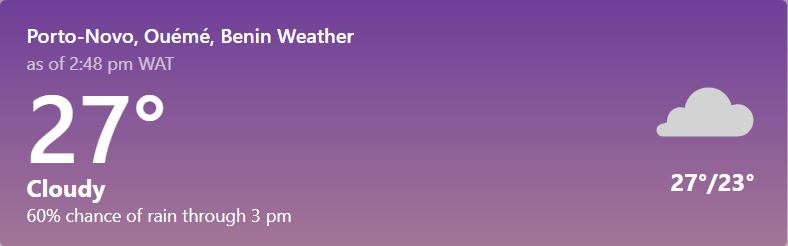
\includegraphics[scale=0.7]{images/benin.JPG}
    \caption{Porto-Novos' weather summary from weather.com}
    \label{fig:benin}
\end{figure}
%
%
Figures \ref{fig:benin}, \ref{fig:vapour}  and \ref{fig:filter} where extracted from \link{www.weather.com} and just constitute a mere example of the process a farmer should follow in order to obtain a more precise weather forecast. Figure \ref{fig:benin}, displays a climate summary from city of Porto-Novo in Benin, Africa. Figure \ref{fig:vapour} and \ref{fig:filter} display a satellite view of Porto-Novo and its surroundings with a water-vapour and an infrared filter respectively. These figures will result only useful for experienced farmers. They must know enough not only to determine the implications of the change in climate along the timeline, but also to know which actions to take in consequence, and last but not least when to take them.
%
\begin{figure}[b!]
    \centering
    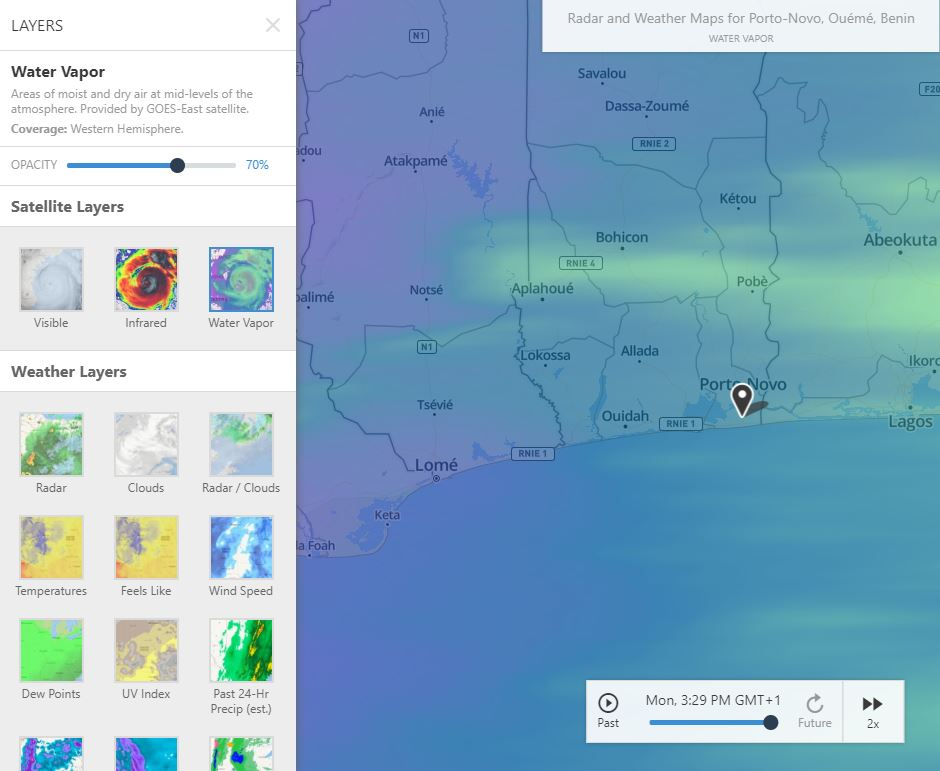
\includegraphics[scale=0.6]{images/water_vapor.JPG}
    \caption{Porto-Novos' satellite image displaying water vapour.}
    \label{fig:vapour}
\end{figure}
\begin{figure}[b!]
    \centering
    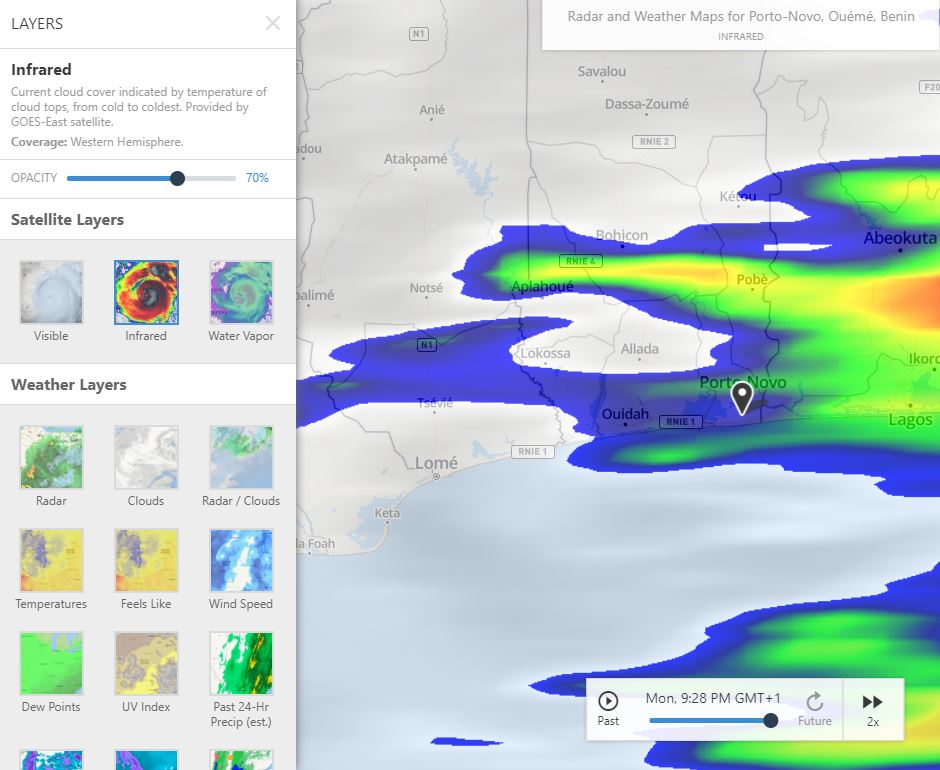
\includegraphics[scale=0.6]{images/infrared.JPG}
    \caption{Porto-Novos' satellite image with an infrared filter.}
    \label{fig:filter}
\end{figure}
\clearpage

\subsection{knowledge of field's characteristics}
Although all farmers know their fields to some extent, not many have precise and/or detailed knowledge about more concrete aspects aspects, e.g. soil height irregularities, chemical characteristics etc. These parameters should be taken into account in order to optimise many farming activities. The major handicap in this aspect is that they are not easy to determine, and in some cases it implies an expensive and time-consuming deployment of measuring devices. ARIFI expects to contribute to this necessity by offering farmers more detailed knowledge of their farms, making use of GNSS services combined with AI and signal/image processing techniques.
\subsection{Adaptation to climate change}
Climate change affects agriculture in particular by changing the intensity and duration of certain meteorologic conditions. This not only affects the way farmers have to manage their fields, but also shifts periodic climate conditions within the year, which threats agricultors' farming schedules. That being said, to optimise their harvest, farmers should not only anticipate threatening climate changes, such as heat waves, but also to adapt their yearly farming schedule to these climate shifts.
ARIFI aims to provide support to farmers in this issue by making thanks to its artificial intelligence module. The latter will keep track of climate distortions over time so as to make more accurate predictions of climate changes and shifts.  
% OVERVIEW
\subsection{Project overview}
%
\begin{figure}[b!]
    \centering
    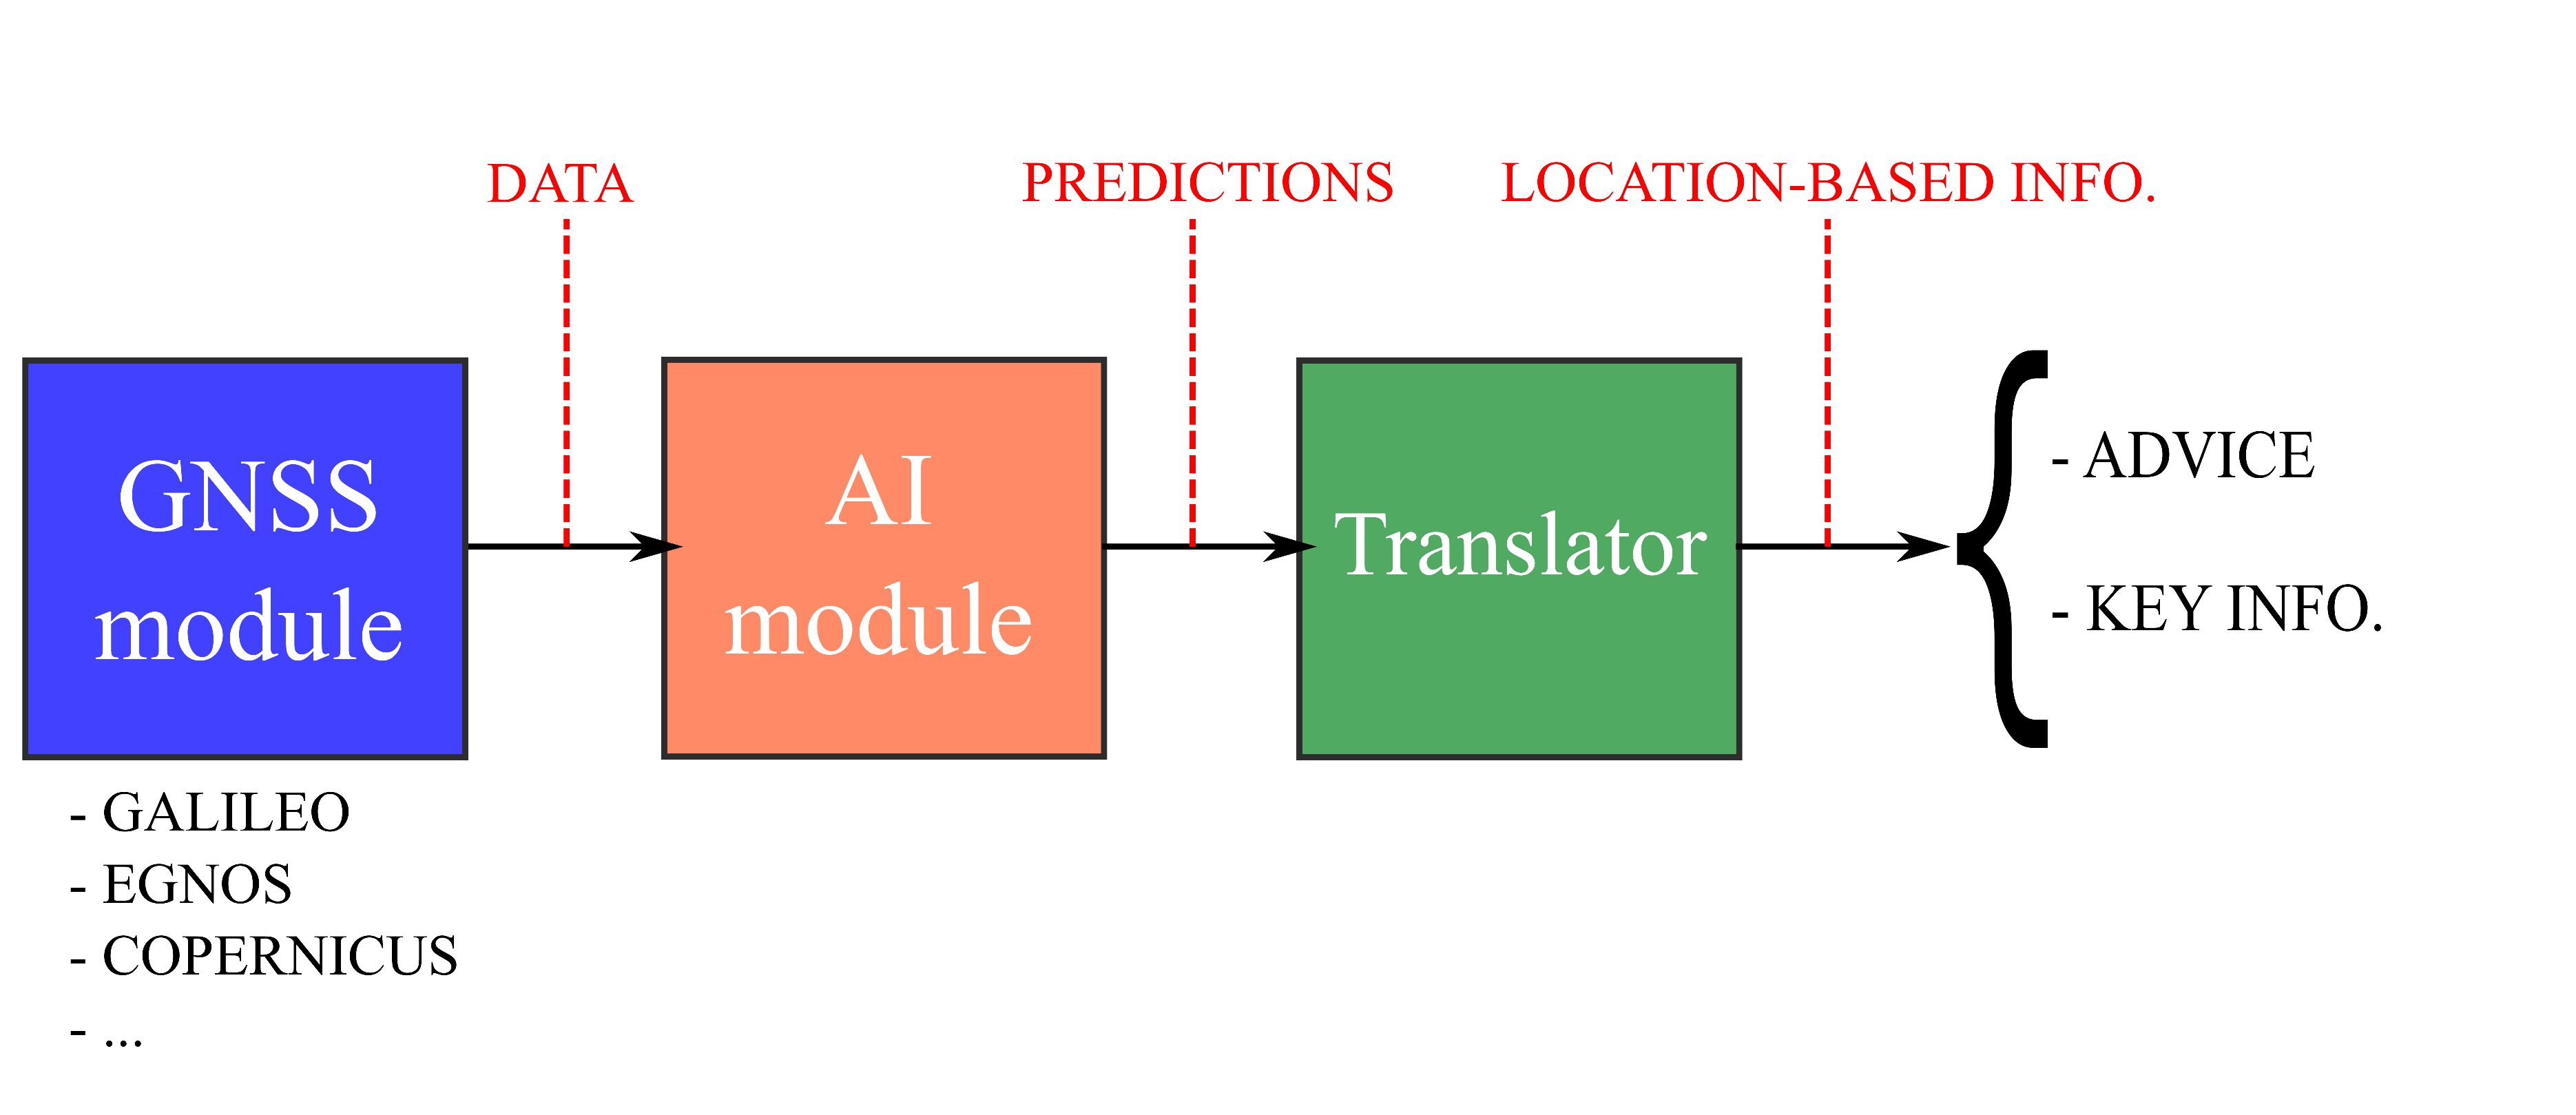
\includegraphics[scale= 0.26]{images/dibujo1.eps}
    \caption{ARIFI's general schematic}
    \label{fig:sch1}
\end{figure}
%
The principal idea is that GNSS together with other sources act as data providers to ARIFI's AI module, which will collect and integrate this information to its algorithm. Next, the AI module will output a prediction of key parameters, that will be later interpreted and made understandable for agricultors. This part is where ARIFI specially stands out from other services, as it will make special emphasis in translating AI predictions into instructions for farmers, so that their harvest follows a more efficient agricultural plan. In figure \ref{fig:sch1}, it is displayed an schematic idea of ARIFI's general concept.\\\\
%
\begin{figure}[t!]
    \centering
    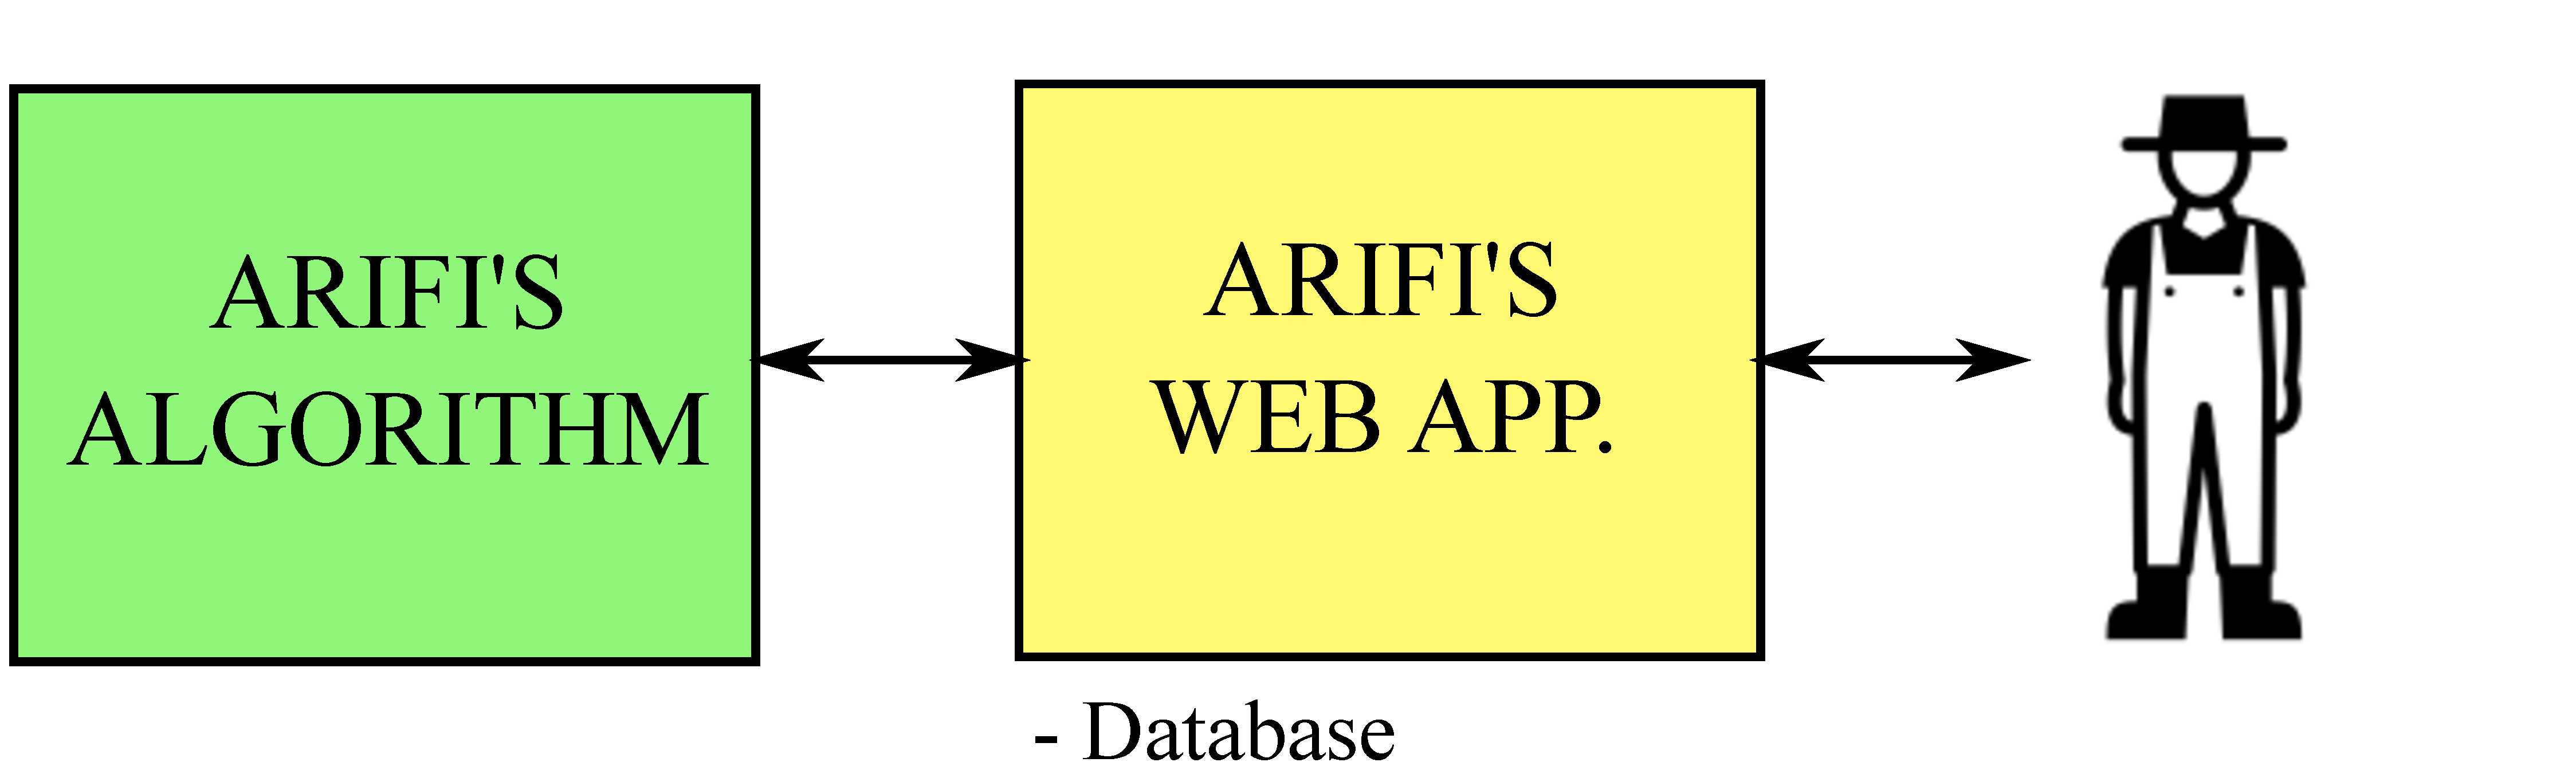
\includegraphics[scale= 0.15]{images/dibujo2.eps}
    \caption{User interaction with ARIFI's services}
    \label{fig:sch2}
\end{figure}
%
ARIFI was initially thought to work as a web application. The reason to this is that one of the major concerns from ARIFI's team, was to make this service available for a wide range of users. With this in mind, a web application was thought the best platform to work with, as it only requires a device with internet connection to access to its services. Despite this, we are opened to consider other platforms such as mobile-phone applications in the future. A graphical description of user's interaction with ARIFI is depicted in figure \ref{fig:sch2}.

\subsection{Technical aspect}
\subsubsection{Satellite services}
\begin{itemize}
    \item \textbf{GALILEO}
    \item \textbf{EGNOS}
    \item \textbf{Copernicus}
    
\end{itemize}
\subsubsection{Artificial intelligence}
To address the proposed idea and achieve our goal, we will focus on how to relate machine learning techniques, field of Artificial Intelligence (AI), with the study of the atmosphere provided by satellite data. Thanks to the Copernicus Atmosphere Monitoring Service, we will be able to access to data that will allow us to predict the main atmospheric phenomenons which affects the production of the majority farmers.\\\\
%
In particular, we are talking about reanalysis variables. This kind of data is obtained by some weather forecasting centres, which combine past observations with a modern meteorological forecast model, in order to produce regular gridded datasets of many atmospheric and oceanic variables, with a temporal resolution of a few hours. This datasets usually extend over several decades and cover the entire planet, being a very useful tool for meteorological and climatological studies.\\\\
%
One of the most important reanalysis projects is the {\em ERA-Interim reanalysis project}, produced by the European Centre for Medium-Range Weather Forecasts (ECMWF) \cite{ERA_Interim}, which belongs to the Copernicus Programme. ERA-Interim is a global atmospheric reanalysis from 1979, continuously updated in real time.\\\\
%
Table \ref{Variables_ERA} is just an example of variables that can be obtained from this platform, which could be used as predictors in machine learning models.

\vspace{12pt}
\begin{table}[H]
\begin{center}
\caption{\label{Variables_ERA} Possible predictive variables in a prediction problem.}
\begin{tabular}{cccc}
\hline
variable name & ERA-Interim variable\\
\hline
\hline
skt & surface temperature\\
sp & surface pression\\
$u_{10}$& zonal wind component ($u$) at 10m\\
$v_{10}$& meridional wind component ($v$) at 10m\\
temp1& Temperature at 500hPa\\
up1& zonal wind component ($u$) at 500hPa\\
\hline
\end{tabular}
\end{center}
\end{table}
\vspace{12pt}

Due to the chaotic nature of atmospheric phenomenons it is so difficult predict with precision its future state. Modeling it without any un- certainty is not possible as there is a strong sensitivity to small perturbations in the initial conditions. But there is a way to overcome this issue by the use of probabilistic weather forecasts \cite{martinez2015forecasting}. In this regard, we propose computational methods belonging to machine learning techniques, a branch of AI, to get predictions or classifications over the main atmospheric factors with high accuracy. We could predict solar radiation, wind velocity, or whatever meteorological process that injures in the farmers' environment. Of course, it would not be possible without GNSS services that provide the essential dataset, as we mentioned before, necessary to train the learning models.

Many of these methods can be classified in the field of Knowledge called “Natural Computing”. The algorithms that can be found in this category are inspired by the way Nature solves complex problems. In this regard, Evolutionary Computation (EC) is inspired in the theory of evolution or Artificial Neural Networks (ANN) find their behaviour in human brain.

The conjunction between satellite data and machine learning algorithms will allow us to provide solutions to those aspects that most concern farmers, in order to keep their harvests safe with the highest possible productivity. For instance, if we are able to anticipate how much water they will have at a given time, or to warn of a dry season that was not previously contemplated but, due to the effects produced by climate change may occur, we will have a positive influence on their economy by avoiding unnecessary expenses derived from poor management, because they do not have all the information they could.

\subsection{Schedule}
ARIFI's project plan follows the GSA Farming by satellite schedule. The latter consists of the 3 phases listed bellow, which have been also displayed in figure X for a more graphical description.
\begin{figure}[b!]
\centering
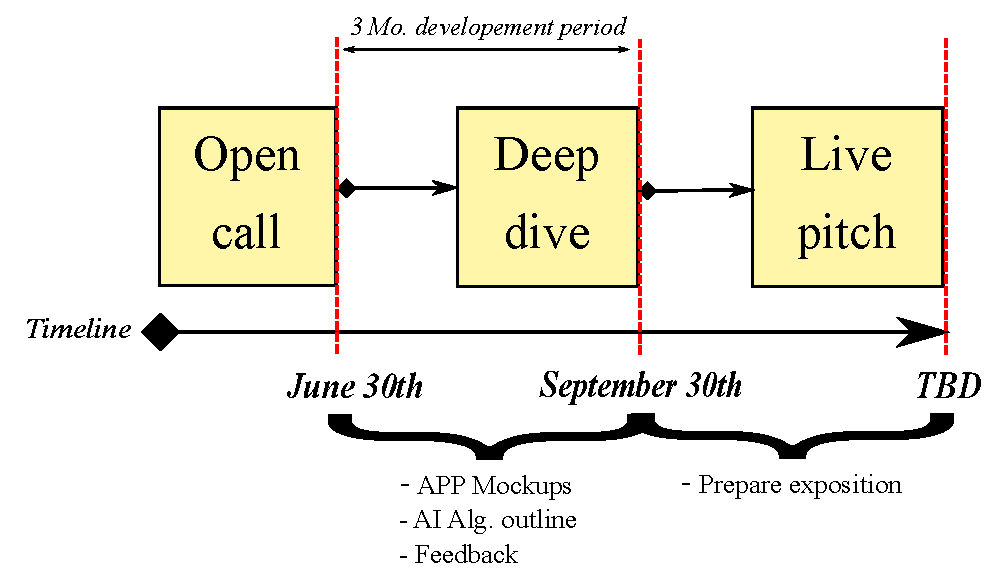
\includegraphics[scale= 0.7]{images/schedule.eps}
\caption{ARIFI's timeline within the GSA contest}
\label{fig:sch2}
\end{figure}
\begin{enumerate}
    \item \textbf{Open call for ideas:} In this phase we worked hard so as to give shape to our project idea. To do this, we kept close contact with our advisory board with a high degree of expertise in agriculture. 
    \item \textbf{Deep Dive Phase:} In this phase we expect to outline more concrete details about ARIFI, also taking advantage from GSA advice. The list of pending subjects we have left for the deep dive phase are the following:
    \begin{itemize}
        \item \textbf{Web Application Interface:} We expect to define a primary web interface so that reviewers can have a feeling of how will the user interaction with the app be. We expect to make an accurate mock-up similar to the final version.
        \item \textbf{AI algorithm:} Our expert in AI has described how should the AI algorithm work so as to output key data, that will later be required from consecutive modules. However, more work is needed in this subject so as to define and adapt more accurately this concrete module to project as a whole.
        \item \textbf{Advisor's supervision:} We do not forget that in order to achieve ARIFI's success, we should keep in constant contact with our advisors and take experts feedback into account, so as to avoid drifting off the initial objective and cover farmer necessities.
    \end{itemize}
    \item \textbf{Live Pitches:} After presenting our work from the deep dive face, we will count with a yet to be determined period of time to create our live pitch exposition and to prepare ARIFI's presentation.\\
\end{enumerate}




% TODOS

\section{The team.}
% JOAN
\begin{wrapfigure}{L}{0.15\textwidth}
        \roundpic[xshift=0cm,yshift=0cm]{2.45cm}{2.45cm}{images/joan.jpg}
    \end{wrapfigure}
\textbf{Joan Bernabeu Frias} is from Barcelona, Spain and was born in 1996. He obtained his BsC in Telecommunications Engineering in 2019 from Autonomous University of Barcelona. He was finalist and winner of two rewards in the 2019 ESA's Galileo APP competition. He is a GNSS pastionate, and is currently working as a Satellite navigation engineer in GMV.\\

% LAURA
\begin{wrapfigure}{L}{0.15\textwidth}
        \roundpic[xshift=0cm,yshift=0cm]{2.45cm}{2.45cm}{images/Laura.png}
    \end{wrapfigure}
\textbf{Laura} is from Madrid, Spain and was born in 1990. She is a Ph.D. Assistant professor in the University of Rey Juan Carlos (Madrid). Doctor Cum Laude by the University of Alcalá in 2018, recognized with the extraordinary doctorate award of the University of Alcalá (2019), her research activity has been focused on the development of different algorithms and techniques belonging to Artificial Intelligence field and their application to different problems in Science and Engineering, especially in those related to renewable energy problems.\\

% SONIA
\begin{wrapfigure}{L}{0.15\textwidth}
        \roundpic[xshift=0cm,yshift=0cm]{2.45cm}{2.45cm}{images/Sonia.jpg}
    \end{wrapfigure}

\textbf{Sonia Framis} is from Barcelona, Spain and was born in 1994. After finishing her Bachelors degrees in Telecommunications Engineering from Universitat Autònoma de Barcelona, Barcelona, Spain, in 2019, she focused on the fields of GNSS and signal processing, in which she is actively pursuing her career. She is currently working on the new generation of the central processing facility of EGNOS in GMV.\\

\newpage
\begin{wrapfigure}{L}{0.15\textwidth}
        \roundpic[xshift=0cm,yshift=0cm]{2.45cm}{2.45cm}{images/Freddy.png}
    \end{wrapfigure}
\textbf{Freddy Pinto Benel} received his Telecommunication Engineer degree from the Universidad de Alcalá (UAH), Spain, in 2013, the M.Sc. and Ph.D. in Information Technology and Communications from the UAH in 2014 and 2019, respectively. Dr. Pinto-Benel held summa cum laude in his doctoral dissertation. Since 2018 he has been working at GMV as signal processing engineer, within the G2G-WO1 project. Since February 2020 he has been leading the signal processing team involved in the development of a DVB-S2 transmitted signal simulator.\\

\subsection{Advisors}\label{adv}
During the first stages of the project, many professionals where reached to get first-hand insight of agriculture's situation. Amongst all of the, the ones presented below proved to be the most proactive and collaborative. They offered themselves to  advise us when doubts arise and to provide their opinion, specially from the farmer-user prospective.\\

\begin{wrapfigure}{L}{0.15\textwidth}
        \roundpic[xshift=0cm,yshift=0cm]{2.45cm}{2.45cm}{images/adv_africa.jpg}
    \end{wrapfigure}
\textbf{Amèhouho Bognon Théodore} is from Benín, Africa. In 2018 he obtained his BsC in Rural Engineering and water management from Université d'Abormey-Calavi and in 2019 his MsC in Digital Agriculture. He has been closely related to agricultural concerns from his region and is now a Research and Development Intern at RADE ONG.\\
%
\newpage
%
\begin{wrapfigure}{L}{0.15\textwidth}
        \roundpic[xshift=0cm,yshift=0cm]{2.45cm}{2.45cm}{images/adv_eu1.jpg}
    \end{wrapfigure}
\textbf{María Dolores Jiménez Ruz} is from Madrid, Spain. She obtained her BsC in 1995 in Agronomous engineering from Universidad de Cordoba. she is an expert in presicion agriculture. In 2015 she started working at HIDROSOPH, a company focused in the design, development and implementation of irrigation and fertilisation systems, assusming the role of technical director and salesman in Spain.\\

\begin{wrapfigure}{L}{0.15\textwidth}
        \roundpic[xshift=0cm,yshift=0cm]{2.45cm}{2.45cm}{images/adv_us.jpg}
    \end{wrapfigure}
\textbf{Lorna G.} is from Hastings, Minnesota. She is an IT systems engineer very passionate about farming. She obtained her certificate from  Oregon State University's master gardener program  in 2020. She is currently a volunteer farmer seeking the goal of creating a self-sustaining 'smart' farm. \\



\begin{thebibliography}{100}

\bibitem{ERA_Interim}
Dick~P Dee, SM~Uppala, AJ~Simmons, Paul Berrisford, P~Poli, S~Kobayashi,
  U~Andrae, MA~Balmaseda, G~Balsamo, P~Bauer, et~al.
\newblock {The ERA-Interim reanalysis: Configuration and performance of the
  data assimilation system}.
\newblock {\em Quarterly Journal of the royal meteorological society},
  137(656):553--597, 2011.

\bibitem{martinez2015forecasting}
G~Mart{\'\i}nez-Arellano.
\newblock {\em Forecasting wind power for the day-ahead market using numerical
  weather prediction models and computational intelligence techniques}.
\newblock PhD thesis, Nottingham Trent University, 2015.

\end{thebibliography}



\end{document}
